\chapter{Describing and Verifying Hardware: RTL, Verilog, Clock Domains and FIFOs}
\label{ch:rtl}

Nobody draws a billion transistors by hand. Digital designers describe hardware in a \term{hardware description language} (HDL), most often Verilog or SystemVerilog, at the \term{register-transfer level} (RTL): registers, and the logic that computes their next values. Tools then turn that description into gates (synthesis) and the gates into layout. This chapter covers the HDL ideas that hardware questions test, two design problems that come up constantly (crossing between clock domains, and sizing FIFOs), and finally how designs are verified before they are built.

\section{An HDL describes hardware, not steps}

Verilog looks like a programming language, but it is not one. A program is a list of steps executed one after another. An HDL describes \emph{circuits that all exist at once}, every gate working in parallel all the time. A line of Verilog does not ``run''; it describes a piece of hardware that is always there.

\section{Verilog in one page}

\begin{lstlisting}[language=Verilog]
module mux2 (
  input  wire       s,
  input  wire [7:0] a, b,     // 8-bit buses, bit 7 is the MSB
  output wire [7:0] y
);
  assign y = s ? b : a;       // continuous assignment: combinational logic
endmodule
\end{lstlisting}

\begin{itemize}
  \item A \code{module} is a block of hardware with \code{input} and \code{output} ports. Modules are instantiated inside other modules to build hierarchy.
  \item \code{[7:0]} declares an 8-bit bus. \code{\{a, b\}} concatenates buses; \code{a[3:0]} selects bits.
  \item \code{assign} describes combinational logic that is always active.
  \item An \code{always @(*)} block also describes combinational logic, using \code{if} and \code{case}.
  \item An \code{always @(posedge clk)} block describes flip-flops: everything assigned inside updates on the rising clock edge.
\end{itemize}

\begin{lstlisting}[language=Verilog]
module counter4 (
  input  wire       clk, rst_n, en,
  output reg  [3:0] count
);
  always @(posedge clk or negedge rst_n) begin
    if (!rst_n)      count <= 4'd0;          // asynchronous, active-low reset
    else if (en)     count <= count + 4'd1;  // count when enabled
  end
endmodule
\end{lstlisting}

(In Verilog, a signal assigned in an \code{always} block is declared \code{reg}; that does not necessarily mean it becomes a register. SystemVerilog replaces both \code{wire} and \code{reg} with \code{logic}. It also adds \code{always\_ff} and \code{always\_comb}, which state the designer's intent, so tools can warn when the code does not really describe flip-flops or pure combinational logic, for example when an \code{always\_comb} block would infer a latch.)

\section{Blocking and nonblocking assignments}
\label{sec:blocking}

Verilog has two assignment operators inside \code{always} blocks, and confusing them is the most famous Verilog bug.

\begin{itemize}
  \item \textbf{Blocking} \code{=}: the assignment happens immediately, and the next statement sees the new value, like a programming language.
  \item \textbf{Nonblocking} \code{<=}: the right-hand sides are all evaluated first, using the old values, and all the left-hand sides are updated together at the end of the time step, like flip-flops all capturing on the same clock edge.
\end{itemize}

\begin{worked}{swapping two registers}
Start with \code{a = 1}, \code{b = 2}.

\textbf{Nonblocking:}
\begin{lstlisting}[language=Verilog]
always @(posedge clk) begin
  a <= b;
  b <= a;
end
\end{lstlisting}
Both right sides use the old values: after the first edge \code{a = 2, b = 1}; after the second \code{a = 1, b = 2}. The registers swap every cycle, which is what two cross-connected flip-flops do.

\textbf{Blocking:}
\begin{lstlisting}[language=Verilog]
always @(posedge clk) begin
  a = b;    // a becomes 2 immediately
  b = a;    // reads the NEW a, so b becomes 2
end
\end{lstlisting}
After the first edge \code{a = 2, b = 2}, and they stay 2 forever. No swap.
\end{worked}

\begin{worked}{what does \code{\$display} print?}
\begin{lstlisting}[language=Verilog]
always @(posedge clk) begin
  a <= b;
  b <= a;
  $display("a=%0d b=%0d", a, b);
end
\end{lstlisting}
With \code{a = 1, b = 2} initially, the first edge prints \code{a=1 b=2}, not the swapped values: nonblocking updates happen at the \emph{end} of the time step, after \code{\$display} has already run. The second edge prints \code{a=2 b=1}.
\end{worked}

\begin{onoa}
A reported question shows an \code{always} block with blocking and nonblocking assignments and asks what values of \code{a} and \code{b} are displayed in the first and second cycles. Work through it as above: blocking updates are seen by the following statements immediately; nonblocking updates are not visible until the time step ends.
\end{onoa}

\begin{remember}
Use \code{<=} (nonblocking) in clocked \code{always @(posedge clk)} blocks. Use \code{=} (blocking) in combinational \code{always @(*)} blocks. Never mix them in one block.
\end{remember}

\section{Accidental latches}

In a combinational \code{always @(*)} block, every output must be assigned a value in \emph{every} path through the code. If some path leaves an output unassigned, the output must ``remember'' its old value, and synthesis creates a latch, usually unintended.

\begin{lstlisting}[language=Verilog]
always @(*) begin
  if (sel) y = a;        // no else: when sel is 0, y must hold its value
end                      //   -> a latch is inferred
\end{lstlisting}
The fix: add the \code{else}, give a \code{default} in every \code{case}, or assign a default value at the top of the block.

\section{Resets}

\paragraph{Synchronous reset.} The reset is just another input to the logic in front of the flip-flops: \code{if (rst) q <= 0;} inside \code{always @(posedge clk)}. It takes effect at the next clock edge, so it needs a running clock, but it never causes timing surprises.

\paragraph{Asynchronous reset.} The reset is in the sensitivity list (\code{always @(posedge clk or negedge rst\_n)}) and drives the flip-flops' clear pins directly, so it works with no clock. The danger is \emph{releasing} it: if reset deasserts close to a clock edge, some flip-flops may leave reset one cycle earlier than others, or go metastable. The standard solution is a \term{reset synchronizer}: assert reset asynchronously, but release it through two flip-flops clocked by the destination clock (``asynchronous assert, synchronous deassert'').

\paragraph{Filtering glitches on a reset line.} A noisy reset input should not reset the chip because of a brief glitch. One simple filter compares the reset with a delayed copy of itself: for an active-low reset, the filtered reset is asserted only when both the input and its delayed copy are low,
\[
  \text{rst\_n}_{\text{filtered}} = \text{rst\_n} \;\text{OR}\; \text{rst\_n}_{\text{delayed}}.
\]
A low glitch shorter than the delay has already ended by the time its delayed copy arrives, so the two are never low together and the OR output stays high.

\begin{worked}{how many buffers?}
Glitches up to 25\,ns must be filtered. Each buffer in the delay chain delays the signal by 2\,ns. The chain delay must exceed the glitch width: $k \times 2 > 25$, so $k = 13$ buffers (26\,ns). In this circuit the OR gate's own delay applies to both inputs equally, so it does not change the count; if a question's circuit puts a gate delay in only one of the two paths, add it to that path's delay.
\end{worked}

\begin{onoa}
A reported question gives a glitch width $N = 25$\,ns, a buffer delay of 2\,ns and an OR-gate delay of 4\,ns, and asks how many buffers are needed to filter glitches of that width or less. The principle is the one above: the delayed path must be longer than the widest glitch to be filtered, counting every delay that lies only on the delayed path.
\end{onoa}

\section{Clock domain crossing}
\label{sec:cdc}

Large chips have many clocks: one for the GPU cores, one for memory, one for each I/O interface. A group of flip-flops on one clock is a \term{clock domain}. A signal passing from one domain to another is a \term{clock domain crossing} (CDC). The receiving domain's clock has no fixed relation to the sender's, so the signal can change at any moment relative to the receiving clock edge, which violates setup or hold and causes metastability (Section~\ref{sec:metastability}).

\paragraph{One bit: the two-flop synchronizer.} Pass the signal through two flip-flops in a row on the receiving clock (Figure~\ref{fig:sync}). The first may go metastable, but it has a full clock period to settle before the second samples it. The probability that it is still unsettled is exponentially small.

\begin{figure}[h]
\centering
\begin{tikzpicture}
  \dbox{s}{(0,0)}{source FF}{1}
  \dbox{a}{(3.2,0)}{sync 1}{1}
  \dbox{b}{(5.8,0)}{sync 2}{1}
  \draw (s-q) -- (a-d); \draw (a-q) -- (b-d);
  \draw (b-q) -- ++(0.7,0) node[right]{safe to use};
  \draw (s-d) -- ++(-0.5,0);
  \draw (s-clk) -- ++(-0.5,0) node[left]{$clk_A$};
  \draw (a-clk) -- ++(-0.3,0) |- (3.0,-0.6) -- (5.5,-0.6) |- (b-clk);
  \draw (3.0,-0.6) -- ++(-0.6,0) node[left]{$clk_B$};
  \draw[dashed,gray] (2.3,-1.0) -- (2.3,2.6);
  \node[font=\scriptsize,gray] at (1.2,2.75) {domain A};
  \node[font=\scriptsize,gray] at (3.6,2.75) {domain B};
\end{tikzpicture}
\caption{A two-flop synchronizer. The signal leaves domain A from a flip-flop (never from raw logic) and is re-timed by two flip-flops on clock B.}
\label{fig:sync}
\end{figure}

Rules that go with it:
\begin{itemize}
  \item The signal must come straight from a flip-flop in the source domain, not from combinational logic, which could glitch.
  \item A short pulse from a fast domain may fall entirely between the slow domain's clock edges and be missed. Stretch it, or convert it into a level that toggles (a ``toggle synchronizer'').
\end{itemize}

\paragraph{Many bits: never synchronize each bit separately.} If a multi-bit value changes, its bits pass through separate synchronizers with slightly different delays, and the receiver can see a mixture of old and new bits, a value that never existed. Safe methods:
\begin{itemize}
  \item \textbf{Gray code}: if the value is a counter, encode it in Gray code (Section~\ref{sec:gray}). Only one bit changes per step, so the receiver sees either the old value or the new one, never garbage.
  \item \textbf{Handshake}: hold the data stable, send a single ``valid'' bit through a synchronizer, and wait for an acknowledgment to come back the same way before changing the data.
  \item \textbf{Asynchronous FIFO}: the general solution for streams of data, described next.
\end{itemize}

\section{FIFOs}

A \term{FIFO} (first in, first out) is a queue: data is written at one end and read out in the same order at the other. It decouples a producer and a consumer that run at different moments or rates.

\paragraph{Structure.} A FIFO is a small memory used as a circular buffer, plus a \term{write pointer} (where the next word goes) and a \term{read pointer} (where the next word comes from). Both advance and wrap around. The FIFO is \term{empty} when the pointers are equal and \term{full} when the write pointer has gone all the way around and caught up with the read pointer. To tell these two cases apart, the pointers get one extra bit: equal including the extra bit means empty; equal except for the extra bit means full.

\paragraph{Asynchronous FIFOs.} When the writer and reader use different clocks, each side must compare its own pointer with the other side's pointer, which crosses a clock domain. The pointers are converted to Gray code and passed through two-flop synchronizers. Because only one bit changes at a time, the synchronized pointer is always a valid (if slightly old) value, and a slightly old value can only make the FIFO look a little fuller or emptier than it is, which is safe.

\section{How deep must a FIFO be?}
\label{sec:fifodepth}

\begin{bigidea}
A FIFO must hold whatever the writer produces faster than the reader can consume. During a burst of $B$ words, the writer takes time $B/r_w$ (where $r_w$ is the write rate in words per second), and in that time the reader removes $r_r \cdot B/r_w$ words. The rest must wait in the FIFO:
\[
  \text{depth} \ge B - B\,\frac{r_r}{r_w} = B\left(1 - \frac{r_r}{r_w}\right).
\]
\end{bigidea}

\begin{worked}{a simple burst}
The writer runs at 100\,MHz and writes one word per cycle in bursts of 120 words. The reader runs at 50\,MHz and reads one word per cycle. Burst time: $120/100\,\text{MHz} = 1.2\,\mu$s. Words read in that time: $1.2\,\mu\text{s} \times 50\,\text{MHz} = 60$. Depth: $120 - 60 = 60$ words.
\end{worked}

\begin{worked}{idle cycles}
The writer runs at 200\,MHz and writes a burst of 100 words, one per cycle. The reader runs at 100\,MHz but can only accept one word every 2 cycles, an effective rate of 50 million words per second. Burst time: $100/200\,\text{MHz} = 0.5\,\mu$s. Words read: $0.5 \times 50 = 25$. Depth: $100 - 25 = 75$ words.
\end{worked}

Real questions add details: idle cycles on the write side (use the effective rate), a worst case where two bursts arrive back to back, or a few extra entries for synchronizer latency in an asynchronous FIFO. Always convert everything to \emph{words per second} first. If the reader is at least as fast as the writer, a FIFO only needs to cover latency, not rate mismatch.

\begin{onoa}
FIFOs are reported on the Ignite assessment, and FIFO depth calculations (module A writing to module B at a different frequency) on other NVIDIA hardware tests. Be ready to explain what a FIFO is, how full and empty are detected, why asynchronous FIFOs use Gray-coded pointers, and how to size one.
\end{onoa}

\section{Handshakes and arbiters}

\paragraph{Valid/ready.} Within one clock domain, blocks usually exchange data with a \term{valid/ready} handshake: the sender raises \code{valid} when it has data; the receiver raises \code{ready} when it can take it; a transfer happens on each clock edge where both are high. This lets either side pause the other (\term{backpressure}).

\paragraph{Arbiters.} When several requesters share one resource (a memory port, a bus), an \term{arbiter} grants it to one at a time. A \term{fixed-priority} arbiter always prefers the lowest-numbered requester, which is simple but can starve the others. A \term{round-robin} arbiter rotates priority after each grant, so every requester is eventually served.

\section{Verification basics}
\label{sec:verif}

Writing RTL is half the job. The other half, usually the larger half, is \term{verification}: showing that the RTL does what the specification says, in every situation it will meet, \emph{before} the chip is manufactured. A bug found in simulation costs an afternoon. A bug found in silicon can cost a new set of manufacturing masks (millions of dollars at advanced nodes) and months of delay, or a product recall. That is why large chip teams often have more verification engineers than designers, and why ``GPU Verification and Design'' is one of the Ignite internship areas.

\begin{bigidea}
Verification asks three questions, again and again: \textbf{Did I drive the design with enough different inputs?} (stimulus) \textbf{Did I check every output for the right answer?} (checking) \textbf{How do I know I have tested enough?} (coverage)
\end{bigidea}

\subsection*{The verification plan}

Before writing any test, a verification engineer reads the specification and writes a \term{verification plan}: a list of every feature and every rule the design must obey, how each will be tested, and what ``tested enough'' means for it. For a FIFO the plan would include: write then read returns the same data in order; \code{full} rises exactly when the FIFO holds \code{DEPTH} words; writing while full is ignored or flagged; reading while empty is ignored or flagged; simultaneous read and write work at every fill level; reset empties it.

\subsection*{Testbenches}

A \term{testbench} is a piece of HDL (or software) that surrounds the \term{design under test} (DUT), drives its inputs and watches its outputs. The testbench never becomes hardware, so it can use every language feature: loops, random numbers, files, classes.

\begin{figure}[h]
\centering
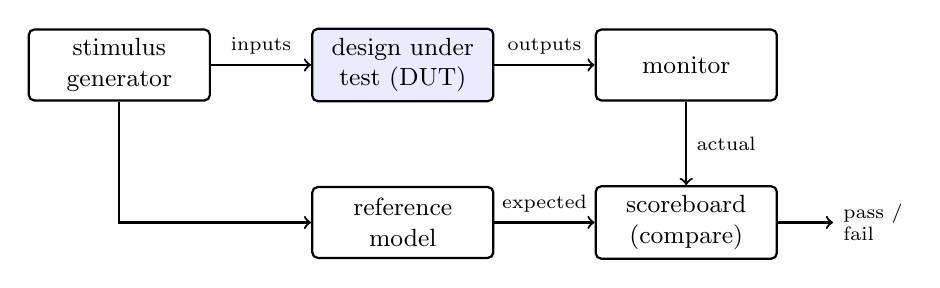
\begin{tikzpicture}[box/.style={draw,thick,rounded corners=2pt,minimum width=2.3cm,minimum height=0.9cm,font=\small,align=center}]
  \node[box] (gen) at (0,0) {stimulus\\generator};
  \node[box,fill=blue!8] (dut) at (3.6,0) {design under\\test (DUT)};
  \node[box] (mon) at (7.2,0) {monitor};
  \node[box] (sb) at (7.2,-2.0) {scoreboard\\(compare)};
  \node[box] (ref) at (3.6,-2.0) {reference\\model};
  \draw[->,thick] (gen) -- node[above,font=\scriptsize]{inputs} (dut);
  \draw[->,thick] (dut) -- node[above,font=\scriptsize]{outputs} (mon);
  \draw[->,thick] (mon) -- node[right,font=\scriptsize]{actual} (sb);
  \draw[->,thick] (gen.south) |- (ref.west);
  \draw[->,thick] (ref) -- node[above,font=\scriptsize]{expected} (sb);
  \draw[->,thick] (sb.east) -- ++(0.7,0) node[right,font=\scriptsize,align=left]{pass /\\fail};
\end{tikzpicture}
\caption{A self-checking testbench. The same stimulus goes to the design and to a reference model; a scoreboard compares what the design did with what it should have done.}
\label{fig:testbench}
\end{figure}

The most important rule: a testbench must \term{check} results automatically. Looking at waveforms by eye works for ten cycles, not for ten million. A \term{self-checking testbench} computes the expected answer itself, from a \term{reference model} (also called a \term{golden model}): a simple, obviously correct description of what the design should do, often written in SystemVerilog, C or Python. The reference model does not need to be fast or synthesizable, only right.

\begin{lstlisting}[language=Verilog]
module tb_adder8;
  logic [7:0] a, b;
  logic [8:0] sum;
  int errors = 0;

  adder8 dut (.a(a), .b(b), .sum(sum));   // the design under test

  task check(input logic [7:0] x, y);
    a = x; b = y;
    #1;                                   // let the logic settle
    if (sum !== x + y) begin              // reference model: the + operator
      errors++;
      $display("FAIL: %0d + %0d gave %0d", x, y, sum);
    end
  endtask

  initial begin
    check(8'd0,   8'd0);                  // directed corner cases first
    check(8'd255, 8'd1);
    check(8'd255, 8'd255);
    repeat (10000) check($urandom, $urandom);   // then random inputs
    $display("%0d errors", errors);
    $finish;
  end
endmodule
\end{lstlisting}

The comparison uses \code{!==}, which also catches \code{X} (unknown) and \code{Z} values on the output; \code{!=} would quietly treat them as ``not different.''

\subsection*{Directed, random and constrained-random tests}

\begin{itemize}
  \item A \term{directed test} applies inputs chosen by hand to exercise one feature or corner case: fill the FIFO exactly to full, add $255 + 1$. Directed tests are easy to understand, but they only find the bugs someone thought of.
  \item \term{Random} stimulus finds the bugs nobody thought of, but purely random inputs are often illegal (a packet length of zero, a misaligned address) or miss rare situations.
  \item \term{Constrained-random} stimulus is random within rules that keep it legal and steer it toward interesting cases. SystemVerilog builds this into the language:
\end{itemize}

\begin{lstlisting}[language=Verilog]
class packet;
  rand bit [7:0]  len;
  rand bit [31:0] addr;
  constraint legal { len inside {[1:64]};        // 1 to 64 bytes
                     addr[1:0] == 2'b00; }        // word-aligned
endclass
\end{lstlisting}

Each run uses a \term{seed} for its random number generator, and the seed is printed, so any failing run can be repeated exactly. Teams run \term{regressions}: thousands of tests with different seeds every night, so that a change that breaks something is caught the next morning.

\subsection*{Assertions}

An \term{assertion} states a rule that must always hold and reports an error the moment it is broken, at the place where the bug happens, not hundreds of cycles later when a wrong value finally reaches an output. SystemVerilog has two kinds:
\begin{itemize}
  \item An \term{immediate assertion} checks a condition at one moment, like an \code{if} that reports an error: \code{assert (count <= DEPTH);}
  \item A \term{concurrent assertion} (SystemVerilog Assertions, SVA) checks a property over clock cycles:
\end{itemize}

\begin{lstlisting}[language=Verilog]
// every request is granted within 1 to 3 cycles
assert property (@(posedge clk) disable iff (!rst_n) req |-> ##[1:3] gnt);

// the FIFO is never written while it is full
assert property (@(posedge clk) disable iff (!rst_n) !(wr_en && full));
\end{lstlisting}

Read \code{|->} as ``implies, starting this cycle'' and \code{\#\#[1:3]} as ``1 to 3 cycles later.'' Assertions are written once and then checked in every test, and formal tools (below) can try to prove them.

\subsection*{Coverage: how do you know you are done?}

Passing tests prove nothing about the situations the tests never reached. \term{Coverage} measures what was reached.
\begin{itemize}
  \item \term{Code coverage} is collected automatically by the simulator: which lines ran (line coverage), which branches of each \code{if} and \code{case} were taken (branch coverage), whether every signal toggled both ways (toggle coverage), and which FSM states and transitions occurred.
  \item \term{Functional coverage} is written by the engineer from the verification plan: did the scenarios that matter actually happen? Was the FIFO ever full? Was it written and read in the same cycle while full? Did every opcode run with a negative operand?
\end{itemize}

\begin{lstlisting}[language=Verilog]
covergroup fifo_cg @(posedge clk);
  level: coverpoint count { bins empty  = {0};
                            bins middle = {[1:DEPTH-1]};
                            bins full   = {DEPTH}; }
  ops:   cross wr_en, rd_en;       // all four write/read combinations
endgroup
\end{lstlisting}

\begin{trap}
100\% code coverage does not mean the design is correct. It means every line \emph{ran}, not that its results were \emph{checked}, and not that every combination of conditions occurred. A line can execute with the wrong answer in a test that has no checker. Coverage measures the stimulus; only checkers and assertions find bugs.
\end{trap}

Verification is ``done'' (\term{coverage closure}) when the plan's coverage goals are met, every test passes across many seeds, and the rate of newly found bugs has dropped to near zero.

\subsection*{Formal verification}

Simulation checks the input sequences you happen to try. \term{Formal verification} uses mathematical tools to prove that a property holds for \emph{every} possible input sequence (usually up to a bounded number of cycles), or to produce a counterexample: a short, exact input sequence that breaks it. It shines on control logic such as arbiters, FIFOs, handshakes and cache-coherence rules, where rare interleavings hide bugs. \term{Equivalence checking} is a related formal technique that proves two versions of a design behave identically, for example the RTL and the gate-level netlist produced by synthesis.

\subsection*{UVM and the bigger picture}

The \term{Universal Verification Methodology} (UVM) is a standard SystemVerilog class library for building large, reusable testbenches. Its pieces map onto Figure~\ref{fig:testbench}: a \term{sequencer} produces transactions (such as ``write 4 bytes to address 0x40''), a \term{driver} turns them into pin wiggles, a \term{monitor} turns pin activity back into transactions, and these three form an \term{agent} for one interface. A \term{scoreboard} compares observed transactions with the reference model. An agent written once for a bus can be reused on every block that uses that bus.

Verification also happens at several levels. Each block is tested on its own (unit level), then blocks together (subsystem), then the whole chip. Gate-level simulation checks the synthesized netlist. Because full-chip simulation is slow, companies also map the design onto \term{emulators} and FPGA prototypes, which run thousands of times faster, so real software and drivers can run on the chip before it exists. Arithmetic units are a classic verification target: Chapter~\ref{ch:arith} describes the corner cases they are checked against.

\begin{remember}
A test without a checker tests nothing. Start every testbench with a reference model and an automatic comparison, add constrained-random stimulus and assertions, and measure functional coverage against a written plan.
\end{remember}

\section{Summary}

\begin{itemize}
  \item HDLs describe parallel hardware. \code{assign} and \code{always @(*)} make combinational logic; \code{always @(posedge clk)} makes flip-flops.
  \item Nonblocking \code{<=} updates all left sides together at the end of the step (use in clocked blocks). Blocking \code{=} updates immediately (use in combinational blocks).
  \item Missing assignments in combinational blocks infer latches.
  \item Asynchronous resets need synchronous release. A delay-and-combine filter rejects reset glitches shorter than the delay.
  \item Single bits cross clock domains through two-flop synchronizers; multi-bit values need Gray code, handshakes or asynchronous FIFOs.
  \item FIFO depth $\ge B(1 - r_r/r_w)$, with rates in words per second.
  \item Verification: a self-checking testbench compares the design against a reference model. Directed tests hit known corner cases; constrained-random tests find the unexpected. Assertions catch rule violations where they happen. Code coverage shows what ran; functional coverage shows which planned scenarios occurred; neither replaces checking. Formal tools prove properties for all inputs.
\end{itemize}

\section{Exercises}

\begin{enumerate}
  \item With \code{a = 3} and \code{b = 7}, what are \code{a} and \code{b} after one clock edge of \code{a = b; b = a;} (blocking)? Of \code{a <= b; b <= a;}?
  \item In the \code{\$display} example of Section~\ref{sec:blocking}, what is printed at the third clock edge?
  \item Will this infer a latch? \code{always @(*) case (sel) 2'b00: y = a; 2'b01: y = b; endcase} How would you fix it?
  \item Why do we use two flip-flops to synchronize a single bit? Why is this not enough for an 8-bit bus?
  \item A writer at 150\,MHz sends bursts of 300 words; a reader at 100\,MHz reads one word per cycle. What FIFO depth is needed?
  \item Why are asynchronous FIFO pointers passed between domains in Gray code?
  \item Glitches up to 15\,ns must be removed from a reset line using 2\,ns buffers. How many buffers are needed?
  \item Give one advantage of a synchronous reset and one of an asynchronous reset.
  \item Write a Verilog module for a 4-bit counter with enable and synchronous active-high reset.
  \item What makes a testbench ``self-checking''? What is a reference model?
  \item Give one strength of directed tests and one of constrained-random tests.
  \item What is the difference between an immediate and a concurrent assertion? Write a concurrent assertion that \code{gnt} is never high unless \code{req} is high in the same cycle.
  \item A block reaches 100\% line coverage. Name two kinds of bug that could still be present.
  \item What can formal verification show that simulation cannot?
\end{enumerate}

\subsection*{Answers}
\begin{enumerate}
  \item Blocking: \code{a = 7}, \code{b = 7}. Nonblocking: \code{a = 7}, \code{b = 3}.
  \item The values have swapped back by then: after two edges \code{a = 1, b = 2}, so the third edge prints \code{a=1 b=2}.
  \item Yes: for \code{sel} values 10 and 11, \code{y} is not assigned, so it must hold its value. Add \code{default: y = 0;} (or assign \code{y} a default before the \code{case}).
  \item The first flip-flop may go metastable; the second gives it a full cycle to resolve, making failures extremely rare. For a bus, the bits may be captured on different cycles, giving a mixed value that never existed.
  \item Burst time $= 300/150\,\text{MHz} = 2\,\mu$s; read in that time $= 200$; depth $= 100$.
  \item Only one bit changes per increment, so a pointer sampled mid-change is either the old or the new value, never a wrong one.
  \item $k \times 2 > 15$, so 8 buffers (16\,ns).
  \item Synchronous: no timing surprises; filtered by the clock. Asynchronous: works without a running clock and acts immediately.
  \item For example:
\begin{lstlisting}[language=Verilog]
module counter4 (input wire clk, rst, en, output reg [3:0] q);
  always @(posedge clk) begin
    if (rst)      q <= 4'd0;
    else if (en)  q <= q + 4'd1;
  end
endmodule
\end{lstlisting}
  \item It computes the expected result itself and compares it with the design's output automatically, reporting any mismatch. A reference model is a simple, trusted description of the correct behaviour (in SystemVerilog, C or Python) that produces those expected results.
  \item Directed: hits a specific corner case on purpose and is easy to debug. Constrained-random: explores many legal combinations nobody thought to write, finding unexpected bugs.
  \item An immediate assertion checks a condition at one instant, like an \code{if}; a concurrent assertion checks a property across clock cycles. For example: \code{assert property (@(posedge clk) gnt |-> req);}
  \item Lines that ran but whose results were never checked (a wrong answer nobody compared), and combinations of conditions that never occurred together (for example, a write and a read in the same cycle while full). Line coverage says nothing about either.
  \item That a property holds for \emph{every} possible input sequence (up to a bound), or an exact counterexample if it does not. Simulation only checks the sequences that were run.
\end{enumerate}
